The primary objective of the Google Books project is to create a digital library
with global accessibility.~Through collaborations with libraries and publishers
worldwide, the project has amassed a collection of over 40 million books in more
than 400 languages. The process of adding a book to the digital library involves
several key steps, such as library registration, on-site visits by logistics
experts, and shipping the books for scanning. Therefore, the development of an
efficient scanning process requires careful planning for optimal efficiency.
Motivated by these real-world challenges, this problem presents a scenario that
resembles the real-world challenges face by the Google Books team.

In the context of this problem, we are presented with a global library system
housing a diverse collection of books, with each library having at most one copy
of these books.~Libraries are characterized by three key factors: the books they
hold, sign-up time, and scanning rate. The sign-up time represents the duration
(measured in days) required for a library to complete the registration process
before it can commence sending books for scanning. The scanning rate indicates
how many books a library can process daily once the sign-up process concludes.

Nonetheless, there are specific constraints associated with these libraries.
Firstly, only one library can be scanned at any given time, irrespective of any
predefined order. Moreover, once the sign-up process commences for a particular
library, it cannot be halted, and as soon as it concludes, that library becomes
immediately available for sending books for scanning. Notably, each book scanned
contributes a designated score; however, this score is counted only once,
regardless of how many times the book is scanned.

The book scanning process, as described, is nevertheless limited by time as
there is a fixed global deadline for library sign-up. Consequently, it is likely
that only a portion of all available libraries will undergo the sign-up process.
Moreover, for the libraries that are already signed up, this deadline restricts
the number of days during which they are allowed to ship books for scanning.

As an illustrative example, refer to~\Cref{fig:bs-example}, which depicts a
possible book scanning process.~The characteristics of the libraries in the
example are detailed in~\Cref{tab:bs-library-properties}. It is important to
note that, in this specific example, the global deadline has been set at 7 days
(inclusive).

\begin{figure}[h]
  \centering
  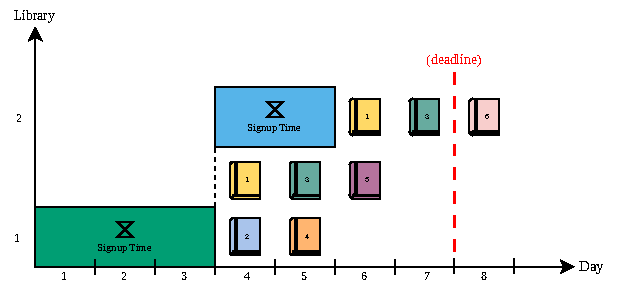
\includegraphics[width=\textwidth,keepaspectratio]{../assets/bs/bs-example.pdf}
  \caption{Book Scanning Process Example}
  \label{fig:bs-example}
\end{figure}

\begin{table}[ht]
  \centering
  \begin{tabular}{cccc}
  \toprule
  Library & Sign-up Time & Rate & Books         \\
  \midrule
  1       & 3            & 2    & 1, 2, 3, 4, 5 \\
  2       & 2            & 1    & 1, 3, 6       \\
  \bottomrule
\end{tabular}
  \caption{Library Properties}
  \label{tab:bs-library-properties}
\end{table}

In this specific example, two libraries have signed up in a non-decreasing order
based on their labels, resulting in a combined sign-up time of 5 days.
Additionally, the scanning rates for these libraries are 2 and 1 for library 1
and 2, respectively. This implies that with this library order, library 1 can
ship a maximum of 8 books, while library 2 can ship 2 books at
most.~Consequently, the latter ends up not contributing one of its books to the
scanning process.~Importantly, this example also highlights a scenario where
both libraries possess duplicate copies of the same books (books 1 and 3).~As
mentioned earlier, these duplicate copies will only be scanned once, regardless
of the number of duplicates, ensuring that they are counted for scoring only
once.

In essence, the objective of this problem is to determine the optimal order for
library sign-ups and book selections for shipping, aiming to maximize the number
of unique books sent for scanning before the deadline. In practical terms, this
translates to maximizing the score awarded by the books that can be scanned.

Mathematically, this can be expressed as shown in~\Cref{eq:objective},
where $\mathcal{B}$ represents the total number of books, $s_{b}$ signifies the
score attributed to scanning book $b$ (for $b = 1, \ldots, \mathcal{B}$), and
$x_{b}$ is a binary variable indicating whether a particular book was shipped
(1) or not (0) by any library.

\begin{equation}
  \label{eq:bs-objective}
  \max{f(s)} = \sum_{b = 1}^{\mathcal{B}}{s_{i} \cdot x_{b}}
\end{equation}

For clarification,~\Cref{ex:bs-problem-scoring} shows an example on how the
objective for this problem is evaluated, given the order for the libraries shown
in~\Cref{fig:bs-example} and the properties exposed in~\Cref{tab:bs-library-properties}.

\begin{example}[Objective Evaluation]
  \label{ex:bs-problem-scoring}
  Consider the books scores presented in~\Cref{tab:bs-example}

  \begin{table}[ht]
    \centering
    \begin{tabular}{ccccccc}
  \toprule
  \textbf{Book}  & 1 & 2 & 3 & 4 & 5 & 6 \\ \midrule
  \textbf{Score} & 3 & 1 & 5 & 4 & 7 & 1 \\
  \bottomrule
\end{tabular}
    \caption{Example Book Scores}
    \label{tab:bs-example}
  \end{table}

  The score obtained for the library scheduling shown in~\Cref{fig:bs-example},
  as determined by the evaluation of the objective~\ref{eq:bs-objective} is~$3 +
    1 + 5 + 4 + 7 = 20$
\end{example}

To conclude, this problem imposes several constraints on various parameters that
describe the book scanning process. The most constraints relevant are shown below:

\begin{description}
  \item[\textbf{$\mathcal{L}$.}] The number of libraries~($ 1 \leq \mathcal{L} \leq 10^5$).
  \item[\textbf{$\mathcal{T}$.}] The number of days required to finish a library sign-up~($ 1 \leq \mathcal{T} \leq 10^5$).
  \item[\textbf{$\mathcal{B}$.}] The number of unique books~($ 1 \leq \mathcal{B} \leq 10^5$).
  \item[\textbf{$\mathcal{N}$.}] The number of books per library~($ 1 \leq \mathcal{N} \leq 10^5$).
  \item[\textbf{$\mathcal{D}$.}] The deadline~($ 0 \leq \mathcal{D} \leq 10^5$).
\end{description}